\documentclass[11pt,a4paper]{article}
\usepackage[margin=22mm]{geometry}
\usepackage{fontspec}
\setmainfont{Latin Modern Roman}
\setsansfont{Latin Modern Sans}
\setmonofont{Latin Modern Mono}
\usepackage{amsmath,amssymb,graphicx,booktabs,longtable,array,calc,etoolbox}
\usepackage[numbers,sort&compress]{natbib}
\usepackage{hyperref,caption,float,fancyvrb}
\hypersetup{hidelinks}
\setcounter{secnumdepth}{-1}
\Urlmuskip=0mu plus 1mu
\RecustomVerbatimEnvironment{verbatim}{Verbatim}{fontsize=\footnotesize}
\DefineVerbatimEnvironment{Highlighting}{Verbatim}{fontsize=\footnotesize}
\providecommand{\tightlist}{\setlength{\itemsep}{0pt}\setlength{\parskip}{0pt}}
\providecommand{\pandocbounded}[1]{#1}
\makeatletter
\def\maxwidth{\ifdim\Gin@nat@width>\linewidth\linewidth\else\Gin@nat@width\fi}
\def\maxheight{\ifdim\Gin@nat@height>.68\textheight .68\textheight\else\Gin@nat@height\fi}
\makeatother
\setkeys{Gin}{width=\maxwidth,height=\maxheight,keepaspectratio}
\AtBeginEnvironment{longtable}{\small}
\renewcommand{\arraystretch}{1.18}
\setlength{\emergencystretch}{3em}
\setlength{\parskip}{4pt}
\setlength{\parindent}{0pt}
\makeatletter
\setlength{\@fptop}{0pt}
\setlength{\@fpsep}{14pt}
\setlength{\@fpbot}{0pt plus 1fil}
\makeatother
\renewcommand{\topfraction}{0.95}
\renewcommand{\bottomfraction}{0.95}
\renewcommand{\textfraction}{0.06}
\renewcommand{\floatpagefraction}{0.80}


\renewcommand{\thefigure}{S\arabic{figure}}
\begin{document}
\hypertarget{supplementary-information}{%
\section{Supplementary Information}\label{supplementary-information}}

\hypertarget{s1-current-c-protocol-and-selected-actors}{%
\subsection{S1 Current C protocol and selected actors}\label{s1-current-c-protocol-and-selected-actors}}

The C prior uses Qwen2.5-VL-7B-Instruct revision cc594898137f460bfe9f0759e9844b3ce807cfb5, P0 without a new system message, clean-plus-R1 image order, bfloat16, SDPA, deterministic generation and at most 500 new tokens. R1 rotates the RGB source clockwise once, limits the longest edge to 1024 pixels and applies readable row-major labels 0-63. A strict parser permits one format repair. The 211-row TRAIN/VALID prior is complete; TEST was not accessed.

\textbf{Table S1. Current C actor selection.}

\begin{longtable}[]{@{}
  >{\raggedright\arraybackslash}p{(\columnwidth - 10\tabcolsep) * \real{0.1304}}
  >{\raggedleft\arraybackslash}p{(\columnwidth - 10\tabcolsep) * \real{0.1739}}
  >{\raggedleft\arraybackslash}p{(\columnwidth - 10\tabcolsep) * \real{0.1739}}
  >{\raggedleft\arraybackslash}p{(\columnwidth - 10\tabcolsep) * \real{0.1739}}
  >{\raggedleft\arraybackslash}p{(\columnwidth - 10\tabcolsep) * \real{0.1739}}
  >{\raggedleft\arraybackslash}p{(\columnwidth - 10\tabcolsep) * \real{0.1739}}@{}}
\toprule\noalign{}
\begin{minipage}[b]{\linewidth}\raggedright
Method
\end{minipage} & \begin{minipage}[b]{\linewidth}\raggedleft
Seed
\end{minipage} & \begin{minipage}[b]{\linewidth}\raggedleft
Selected update
\end{minipage} & \begin{minipage}[b]{\linewidth}\raggedleft
VALID A (MPa)
\end{minipage} & \begin{minipage}[b]{\linewidth}\raggedleft
Logical updates
\end{minipage} & \begin{minipage}[b]{\linewidth}\raggedleft
Actual updates
\end{minipage} \\
\midrule\noalign{}
\endhead
\bottomrule\noalign{}
\endlastfoot
C spatial feedback (main) & 2026091301 & 250 & 45.847 & 1250 & 1250 \\
C spatial open-loop & 2026091303 & 1250 & 44.907 & 1250 & 1250 \\
C mean feedback & 2026091305 & 250 & 44.926 & 1250 & 1250 \\
\end{longtable}

All five candidate checkpoints per C actor remain archived. Selection retained the earliest candidate unless a later domain-equal area improved by more than 1e-12. The six controls are frozen historical rows, while the three A policies are stored separately from the 650-row primary matrix.

\hypertarget{s2-statistical-estimands}{%
\subsection{S2 Statistical estimands}\label{s2-statistical-estimands}}

Same-cost endpoint losses first average Random repeat losses within each physical specimen. Pooled MAE and RMSE then aggregate 50 physical specimens. A and early A instead average repeats within specimen, specimens within domain and the six domains equally. Capture-group bootstrap intervals use 5000 paired draws within domain with seed 2026091401. These intervals are exploratory and conditional on checkpoint selection.

Timing uses \(g_t=(1-c_t/0.25)(e_{t-1}-e_t)\) in four right-closed completion intervals. Negative terms are retained and the machine-readable evidence verifies \(A=e_0-\sum_t g_t\). Equal-quality analysis searches the earliest supported crossing on the five-cap and event-union grids; it retains unreached targets, recrossings and negative or undefined savings.

\hypertarget{s3-complete-same-cost-results}{%
\subsection{S3 Complete same-cost results}\label{s3-complete-same-cost-results}}

\begin{longtable}[]{@{}
  >{\raggedright\arraybackslash}p{(\columnwidth - 12\tabcolsep) * \real{0.1111}}
  >{\raggedleft\arraybackslash}p{(\columnwidth - 12\tabcolsep) * \real{0.1481}}
  >{\raggedleft\arraybackslash}p{(\columnwidth - 12\tabcolsep) * \real{0.1481}}
  >{\raggedleft\arraybackslash}p{(\columnwidth - 12\tabcolsep) * \real{0.1481}}
  >{\raggedleft\arraybackslash}p{(\columnwidth - 12\tabcolsep) * \real{0.1481}}
  >{\raggedleft\arraybackslash}p{(\columnwidth - 12\tabcolsep) * \real{0.1481}}
  >{\raggedleft\arraybackslash}p{(\columnwidth - 12\tabcolsep) * \real{0.1481}}@{}}
\toprule\noalign{}
\begin{minipage}[b]{\linewidth}\raggedright
Method
\end{minipage} & \begin{minipage}[b]{\linewidth}\raggedleft
Cap
\end{minipage} & \begin{minipage}[b]{\linewidth}\raggedleft
MAE
\end{minipage} & \begin{minipage}[b]{\linewidth}\raggedleft
RMSE
\end{minipage} & \begin{minipage}[b]{\linewidth}\raggedleft
R2
\end{minipage} & \begin{minipage}[b]{\linewidth}\raggedleft
Mean actual cost
\end{minipage} & \begin{minipage}[b]{\linewidth}\raggedleft
Actual range
\end{minipage} \\
\midrule\noalign{}
\endhead
\bottomrule\noalign{}
\endlastfoot
Center-first & 0.000 & 58.551 & 75.778 & 0.429 & 0.000 & 0.000000-0.000000 \\
Center-first & 0.062 & 47.885 & 64.882 & 0.581 & 0.062 & 0.061399-0.062407 \\
Center-first & 0.125 & 48.827 & 65.932 & 0.568 & 0.111 & 0.109491-0.125000 \\
Center-first & 0.188 & 49.094 & 66.277 & 0.563 & 0.173 & 0.171900-0.187121 \\
Center-first & 0.250 & 48.027 & 65.223 & 0.577 & 0.235 & 0.234676-0.235577 \\
Geometry-spread & 0.000 & 58.551 & 75.778 & 0.429 & 0.000 & 0.000000-0.000000 \\
Geometry-spread & 0.062 & 50.221 & 67.804 & 0.543 & 0.062 & 0.061399-0.062130 \\
Geometry-spread & 0.125 & 46.189 & 62.421 & 0.612 & 0.125 & 0.123164-0.124629 \\
Geometry-spread & 0.188 & 46.555 & 62.347 & 0.613 & 0.187 & 0.186034-0.187407 \\
Geometry-spread & 0.250 & 46.910 & 62.278 & 0.614 & 0.250 & 0.249269-0.250000 \\
Serpentine & 0.000 & 58.551 & 75.778 & 0.429 & 0.000 & 0.000000-0.000000 \\
Serpentine & 0.062 & 49.731 & 64.721 & 0.583 & 0.062 & 0.062130-0.062407 \\
Serpentine & 0.125 & 48.773 & 64.778 & 0.583 & 0.125 & 0.124260-0.124629 \\
Serpentine & 0.188 & 48.343 & 63.931 & 0.593 & 0.187 & 0.186391-0.186851 \\
Serpentine & 0.250 & 48.013 & 63.041 & 0.605 & 0.249 & 0.248521-0.249258 \\
Random & 0.000 & 58.551 & 75.778 & 0.429 & 0.000 & 0.000000-0.000000 \\
Random & 0.062 & 53.156 & 69.115 & 0.525 & 0.054 & 0.046897-0.062500 \\
Random & 0.125 & 49.153 & 65.038 & 0.579 & 0.119 & 0.109307-0.125000 \\
Random & 0.188 & 48.108 & 63.412 & 0.600 & 0.187 & 0.171598-0.187500 \\
Random & 0.250 & 46.886 & 61.941 & 0.618 & 0.247 & 0.234492-0.250000 \\
Learned-static & 0.000 & 58.551 & 75.778 & 0.429 & 0.000 & 0.000000-0.000000 \\
Learned-static & 0.062 & 46.465 & 62.720 & 0.609 & 0.062 & 0.062130-0.062500 \\
Learned-static & 0.125 & 48.064 & 63.994 & 0.593 & 0.125 & 0.124260-0.125000 \\
Learned-static & 0.188 & 46.784 & 62.570 & 0.611 & 0.187 & 0.187130-0.187500 \\
Learned-static & 0.250 & 46.993 & 62.168 & 0.616 & 0.235 & 0.234674-0.249991 \\
No-VLM spatial feedback & 0.000 & 58.551 & 75.778 & 0.429 & 0.000 & 0.000000-0.000000 \\
No-VLM spatial feedback & 0.062 & 43.324 & 60.878 & 0.631 & 0.058 & 0.046897-0.062500 \\
No-VLM spatial feedback & 0.125 & 43.164 & 60.169 & 0.640 & 0.120 & 0.109120-0.124998 \\
No-VLM spatial feedback & 0.188 & 42.928 & 58.388 & 0.661 & 0.183 & 0.171415-0.187407 \\
No-VLM spatial feedback & 0.250 & 42.385 & 56.534 & 0.682 & 0.247 & 0.234492-0.250000 \\
C mean feedback & 0.000 & 58.551 & 75.778 & 0.429 & 0.000 & 0.000000-0.000000 \\
C mean feedback & 0.062 & 44.512 & 62.520 & 0.611 & 0.060 & 0.046789-0.062407 \\
C mean feedback & 0.125 & 45.494 & 62.573 & 0.611 & 0.123 & 0.109489-0.124998 \\
C mean feedback & 0.188 & 44.242 & 61.218 & 0.627 & 0.185 & 0.171598-0.187407 \\
C mean feedback & 0.250 & 44.066 & 60.593 & 0.635 & 0.248 & 0.234492-0.250000 \\
C spatial feedback (main) & 0.000 & 58.551 & 75.778 & 0.429 & 0.000 & 0.000000-0.000000 \\
C spatial feedback (main) & 0.062 & 46.987 & 63.404 & 0.600 & 0.060 & 0.046897-0.062407 \\
C spatial feedback (main) & 0.125 & 44.840 & 60.087 & 0.641 & 0.122 & 0.109120-0.124816 \\
C spatial feedback (main) & 0.188 & 44.270 & 59.570 & 0.647 & 0.185 & 0.171898-0.187407 \\
C spatial feedback (main) & 0.250 & 43.711 & 57.756 & 0.668 & 0.248 & 0.234492-0.249999 \\
C spatial open-loop & 0.000 & 58.551 & 75.778 & 0.429 & 0.000 & 0.000000-0.000000 \\
C spatial open-loop & 0.062 & 44.710 & 60.238 & 0.639 & 0.060 & 0.046713-0.062407 \\
C spatial open-loop & 0.125 & 44.720 & 59.192 & 0.651 & 0.122 & 0.109120-0.124814 \\
C spatial open-loop & 0.188 & 43.962 & 58.034 & 0.665 & 0.185 & 0.171898-0.187500 \\
C spatial open-loop & 0.250 & 43.917 & 58.523 & 0.659 & 0.249 & 0.234492-0.250000 \\
\end{longtable}

\hypertarget{s4-historical-a-and-current-c}{%
\subsection{S4 Historical A and current C}\label{s4-historical-a-and-current-c}}

\begin{longtable}[]{@{}
  >{\raggedright\arraybackslash}p{(\columnwidth - 10\tabcolsep) * \real{0.1304}}
  >{\raggedleft\arraybackslash}p{(\columnwidth - 10\tabcolsep) * \real{0.1739}}
  >{\raggedleft\arraybackslash}p{(\columnwidth - 10\tabcolsep) * \real{0.1739}}
  >{\raggedleft\arraybackslash}p{(\columnwidth - 10\tabcolsep) * \real{0.1739}}
  >{\raggedleft\arraybackslash}p{(\columnwidth - 10\tabcolsep) * \real{0.1739}}
  >{\raggedleft\arraybackslash}p{(\columnwidth - 10\tabcolsep) * \real{0.1739}}@{}}
\toprule\noalign{}
\begin{minipage}[b]{\linewidth}\raggedright
Method
\end{minipage} & \begin{minipage}[b]{\linewidth}\raggedleft
Metric
\end{minipage} & \begin{minipage}[b]{\linewidth}\raggedleft
Historical A
\end{minipage} & \begin{minipage}[b]{\linewidth}\raggedleft
Current C
\end{minipage} & \begin{minipage}[b]{\linewidth}\raggedleft
A - C
\end{minipage} & \begin{minipage}[b]{\linewidth}\raggedleft
95\% interval
\end{minipage} \\
\midrule\noalign{}
\endhead
\bottomrule\noalign{}
\endlastfoot
C spatial feedback (main) & area\_mpa & 45.110 & 45.847 & -0.736 & {[}-2.946, 1.455{]} \\
C spatial feedback (main) & early\_area\_mpa & 49.642 & 50.339 & -0.696 & {[}-4.500, 3.118{]} \\
C spatial feedback (main) & endpoint\_abs\_error\_mpa & 44.286 & 43.711 & 0.575 & {[}-1.035, 2.450{]} \\
C spatial open-loop & area\_mpa & 46.501 & 44.907 & 1.594 & {[}-0.500, 3.720{]} \\
C spatial open-loop & early\_area\_mpa & 51.048 & 49.154 & 1.894 & {[}-0.977, 5.090{]} \\
C spatial open-loop & endpoint\_abs\_error\_mpa & 44.822 & 43.917 & 0.905 & {[}-1.122, 2.839{]} \\
C mean feedback & area\_mpa & 45.263 & 44.926 & 0.337 & {[}-2.208, 2.988{]} \\
C mean feedback & early\_area\_mpa & 50.390 & 48.657 & 1.733 & {[}-1.727, 5.652{]} \\
C mean feedback & endpoint\_abs\_error\_mpa & 43.611 & 44.066 & -0.455 & {[}-3.146, 2.411{]} \\
\end{longtable}

Positive A-minus-C values favour current C. All domain-specific values, endpoint paired contrasts and target grids are retained in the accompanying CSV files.

\hypertarget{s5-current-c-case-illustrations}{%
\subsection{S5 Current C case illustrations}\label{s5-current-c-case-illustrations}}

The three cases were fixed before this retraining release. Every panel below was regenerated from the selected current C main-policy trajectory and current C prior. They are process illustrations rather than independent replications.

\begin{figure}[H]
\centering
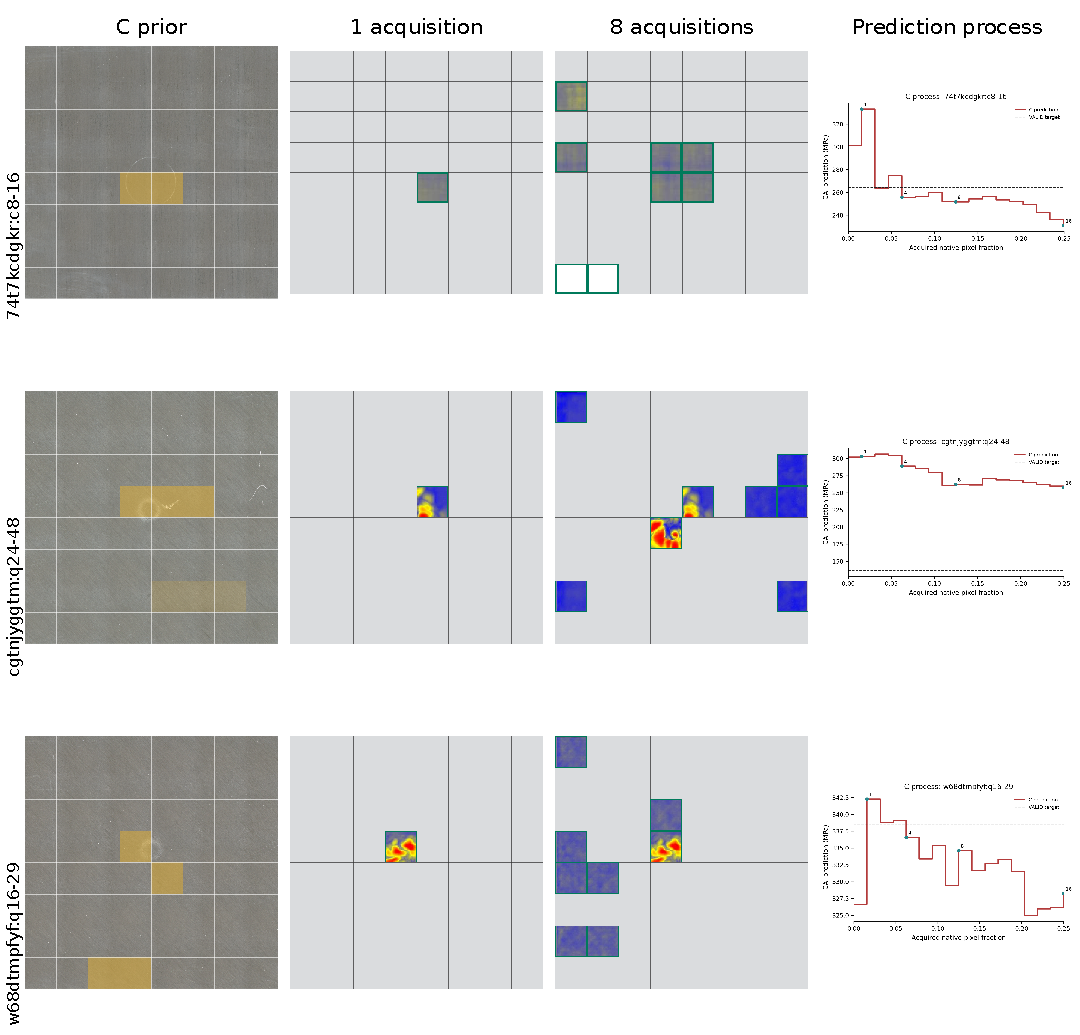
\includegraphics[width=1\textwidth,height=\textheight]{figures/F6_case_progression.pdf}
\caption{Current C candidate surfaces, acquired states and prediction processes for c8-16, q24-48 and q16-29.}
\end{figure}

\hypertarget{s6-source-data-index}{%
\subsection{S6 Source-data index}\label{s6-source-data-index}}

The tables directory contains the recomputed method summary, all five-cap metrics, domain metrics, paired contrasts, A/C version comparisons, event curves, timing contributions, quality targets, case states and full-input reference. The evidence manifest records their hashes. The figures directory contains vector PDF/SVG files and 300-dpi PNG previews, plus all new case PNGs.

\bibliographystyle{unsrtnat}
\bibliography{references}
\end{document}
